% 本科毕业论文选项
\documentclass[bachelor,winfonts]{jnuthesis} %Font: winfonts, sourcefonts, adobefonts.
%\input{bachelor-common}
\usepackage[math]{blindtext}
\usepackage[version=4]{mhchem}
%\usepackage{subfigure}
%\graphicspath{{Figure/}}
\titlea{含硒表面活性剂囊泡的构筑}
\titleb{与性质研究}
\author{陈育明}
\studentnum{1050115220}
\supervisor{刘雪锋}
\supervisorpos{教授}
\supervisorb{}
\supervisorbpos{}
\major{应用化学}
\department{化学与材料工程}
\institute{江南大学}
% 学士学位获得日期,需设置年、月,默认为编译日期。
\bachelordegreeyear{2019}
\bachelordegreemonth{6}

\begin{document}
    % 制作中文封面
    \maketitle
    % 开始前言部分
    \frontmatter
    % 论文的中文摘要
    \begin{abstract}
        复杂网络的研究可上溯到20世纪60年代对ER网络的研究。90年后代随着Internet
        的发展,以及对人类社会、通信网络、生物网络、社交网络等各领域研究的深入,
        发现了小世界网络和无尺度现象等普适现象与方法。对复杂网络的定性定量的科
        学理解和分析,已成为如今网络时代科学研究的一个重点课题。
        \keywords{小世界理论;网络模型;数据中心}
    \end{abstract}
    
    % 论文的英文摘要
    \begin{englishabstract}
        \blindtext
        % 英文关键词。关键词之间用英文半角逗号隔开,末尾无符号。
        \englishkeywords{Small World, Network Model, Data Center}
    \end{englishabstract}
    
    % 生成论文目次
    \tableofcontents
    
    % 开始正文部分
    \mainmatter
    
    \chapter{绪论}\label{chapter_introduction}
    \section{引言}
    表面活性剂因其乳化、润湿、增溶等优良作用而广泛应用于诸如原油回收、土壤修复、乳液聚合、
    药物制备等领域\cite{秦勇2009}。一般情况下,表面活性剂大多具有性能稳定的特点,但在
    大多数情况下,它只在某一阶段起作用,过程结束后,往往分离困难,另一方面,表面活性剂
    一般不参与化学反应,直接排放既是一种浪费,同时给环境带来压力\cite{秦勇2009}。
    
    为应对传统表面活性剂生物降解速率慢,人们发展出可分解表面活性剂(Cleavable Surfactants)
    ,此类表面活性剂在酶、酸碱、光照、加热等条件下可促发分解\cite{hellberg2000}。20世纪80年代
    以来,各种触发机制的开关表面活性剂(Switchable Surfactants)被发展出来,用于调控
    表面活性剂性质,例如,聚合物的乳胶悬浮液在储存运输中需要是稳定的,担当其被施工涂到
    表面之后并不需要稳定的悬浮液,那么能够对这一性质进行“关闭”显然是此类表面活性剂的
    有点\cite{jessop2012}。同时,开关表面活性剂这种“关闭”是可以通过另一种手段进行恢复的。
    本文将简述可分解表面活性剂及其应用的概况,并就刺激手段为分类方式概述开关表面活性剂的发展状况。
    
    \section{可分解表面活性剂}
    可分解表面活性剂最初主要是为了解决环境问题而发展起来的,理论设想通过在分子中嵌入
    易断裂化学键提高生物降解速率,尽管研究中所发现的高效酶催化或化学催化分解未必
    总能够反映到实际中微生物的高效降解\cite{tehrani2007}。传统表面活性剂一般相对稳定,
    早在可分解表面活性剂概念发展之前,季铵酯类表面活性剂已用作纺织品柔软剂,其便是典型的
    可分解表面活性剂。此外,十二烷基硫酸钠的自催化降解、脂肪酸聚氧乙烯酯应当在中性或
    弱碱性使用、羰基表面活性剂酸性条件可分解均被人们注意并用以实际\cite{tehrani2007}。
    而对于可分解表面活性剂,其可采用酶催化分解,也可采用酸催化、碱催化水解或是UV光照、
    臭氧以及加热等手段进行分解,可分解表面活性剂主要包含对酸不稳定(缩醛类、缩酮类、
    原酸酯类及硅氧烷基表面活性剂)、对碱不稳定(季铵酯、甜菜碱酯、单烷基(醚)碳酸酯)以及
    对UV-光照、热及臭氧不稳定的各类表面活性剂,相关文献\cite{hellberg2000,tehrani2007,shukla2010,narayanan2008}对此
    进行了综述,各类型代表可分解表面活性剂见图\ref{fig:cleavable-saa} or 图\ref{fig:cleavable-a}。
    
%    \begin{figure}
%        \centering
%        \subfloat[][]{%
%        \label{fig:cleavable-a}%
%        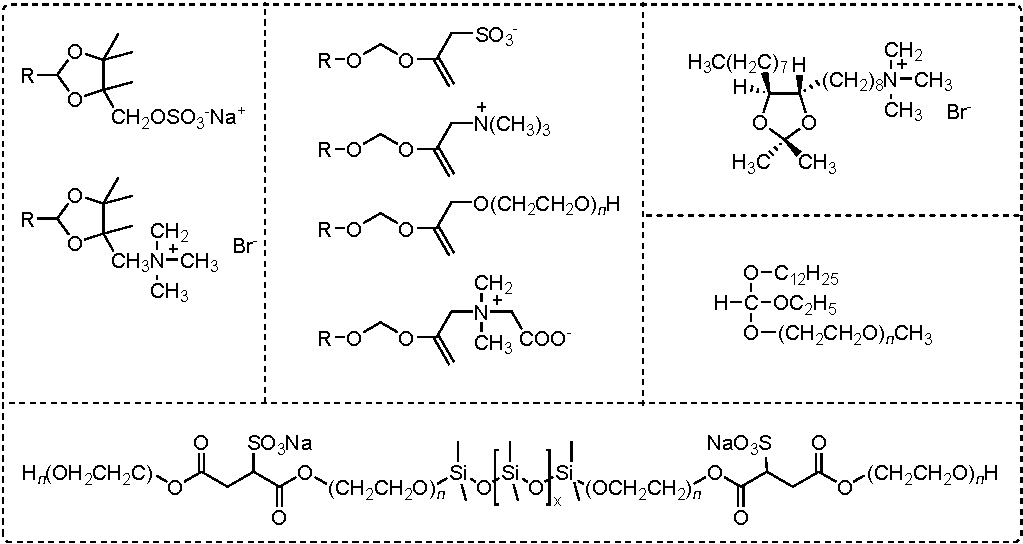
\includegraphics[width=.9\textwidth]{Figure/cleavable-a.png}}%
%        %\hspace{8pt}%
%        \subfloat[][]{%
%        \label{fig:ex3-b}%
%        \includegraphics[width=.9\textwidth]{example-image}}\\
%        \subfloat[][]{%
%        \label{fig:ex3-c}%
%        \includegraphics[width=.9\textwidth]{example-image}}%
%       % \hspace{8pt}%
%        \subfloat[][]{%
%        \label{fig:ex3-d}%
%        \includegraphics[width=.9\textwidth]{example-image}}%
%        \caption[A set of four sub-floats.]{A set of four sub-floats:
%        \subref{fig:cleavable-a} 对酸性不稳定的可分解表面活性剂;
%        \subref{fig:ex3-b} describes the second sub-float;
%        \subref{fig:ex3-c} describes the third sub-float; and,
%        \subref{fig:ex3-d} describes the last sub-float.}%
%        \label{fig:ex3}%
%    \end{figure}
    
    \begin{figure}
        \centering
        \begin{subfigure}[b]{\textwidth}
            \centering
            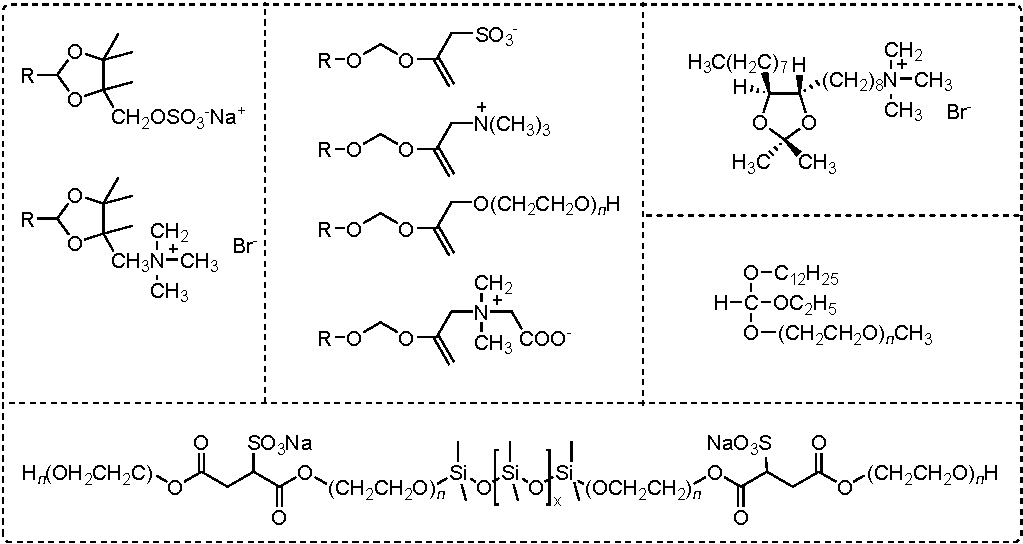
\includegraphics[width=\textwidth]{Figure/cleavable-a.pdf}
            \caption{对酸性不稳定的可分解表面活性剂}\label{fig:cleavable-a}
        \end{subfigure}%
    
        \begin{subfigure}[b]{\textwidth}
            \centering
            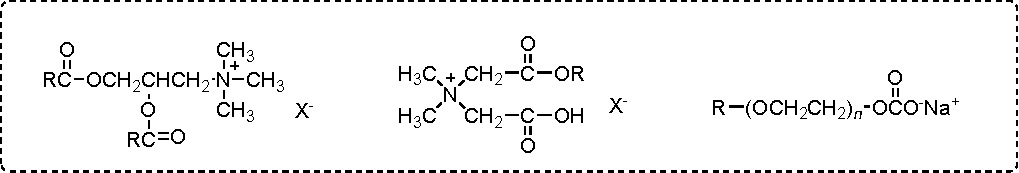
\includegraphics[width=\textwidth]{Figure/cleavable-b.pdf}
            \caption{对碱性不稳定的可分解表面活性剂}\label{fig:cleavable-b}
        \end{subfigure}
    
        \begin{subfigure}[b]{\textwidth}
            \centering
            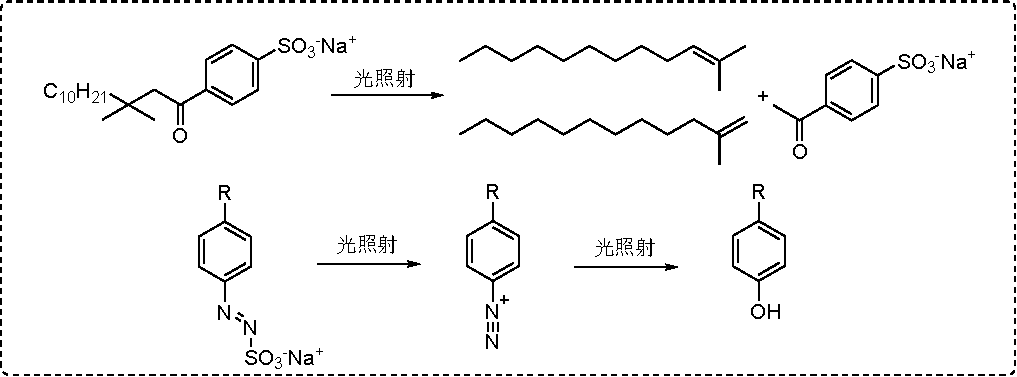
\includegraphics[width=\textwidth]{Figure/cleavable-c.pdf}
            \caption{光照分解表面活性剂}\label{fig:cleavable-c}
        \end{subfigure}%

        \begin{subfigure}[b]{\textwidth}
            \centering
            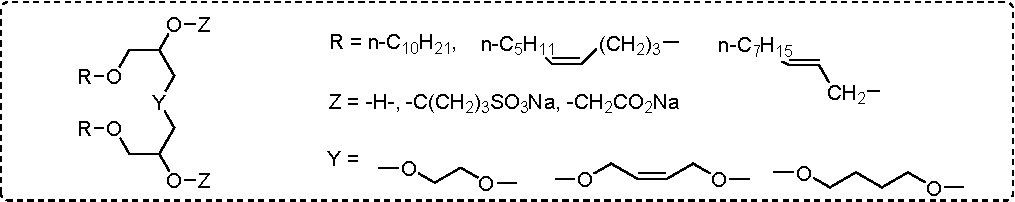
\includegraphics[width=\textwidth]{Figure/cleavable-d.pdf}
            \caption{臭氧分解表面活性剂}\label{fig:cleavable-d}
        \end{subfigure}
    \end{figure}
\addtocounter{figure}{-1} % 将图的编号减1
\begin{figure}[t]
\addtocounter{subfigure}{1} % 子图编号加2
        \begin{subfigure}[b]{\textwidth}
            \centering
            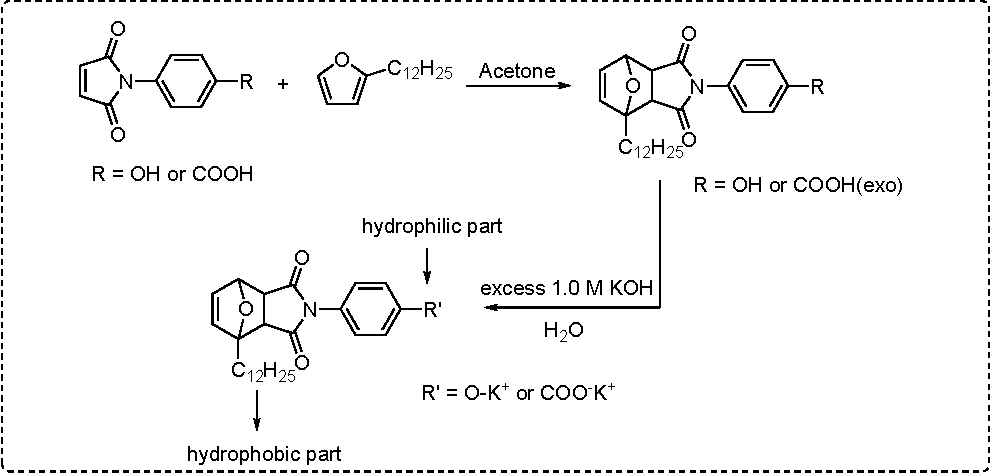
\includegraphics[width=\textwidth]{Figure/cleavable-e.pdf}
            \caption{臭氧分解表面活性剂}\label{fig:cleavable-e}
        \end{subfigure}
        \caption{已发展的可分解表面活性剂类型}\label{fig:cleavable-saa}
    \end{figure}
    e. 通过Diels-Alder反应合成的热不稳定可分解表面活性剂
    
    可分解表面活性剂发展的最初目的是为了解决传统表面活性剂难生物降解的环境问题,同时
    可分解表面活性剂也可在乳化阶段之后通过刺激手段使乳液破乳,也可用于纳米粒子及聚合物制备中
    易脱除的模板剂\cite{liu2007}。此外,一些研究将分解表面活性剂用于膜蛋白的质谱分析\cite{norris2003}
    及胶束电动色谱\cite{stanley2012}。但与此同时,化学或酶催化降解有时不能完全适合于微生物的
    降解\cite{tehrani2007},或是降解速率不高,更重要的一点是其分解过程不可逆\cite{liu2007}。
    
    可分解表面活性剂研究较早,最主要面向解决传统表面活性剂的生物降解问题,已有PPS、ProteaseMAX、
    RapiGest SF等商品化洗涤产品应用可分解表面活性剂。此外,可分解表面活性剂在生物化学、
    医药制造等领域也可有所应用\cite{hellberg2000}。Liu等\cite{guo2012}以氯化肉豆蔻酰胆碱
    (及一种季铵酯表面活性剂,在酶催化或碱催化下可分解)及对磺酸杯芳烃(SC4A)构建二级囊泡,
    利用氯化肉豆蔻酰胆碱在丁酰胆碱酯酶(BChE)作用下酯键断裂,或可应用于阿尔茨海默症的载药及释放(见图\ref{fig:Ch1-SC4A})。
    
    \begin{figure}[htbp]
        \centering
        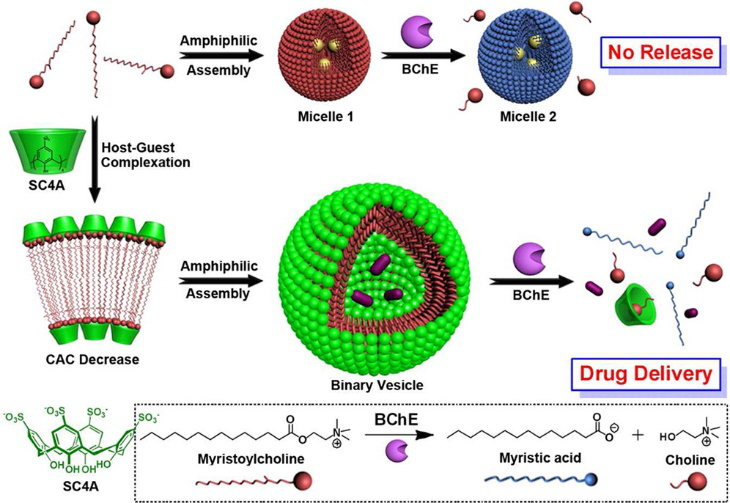
\includegraphics[width= 0.55\textwidth]{Figure/Ch1-SC4A}\\
        \caption{肉豆蔻酰胆碱在SC4A空白及存在下的两亲自组装示意图}\label{fig:cleavale-SC4A}
    \end{figure}
        
        \begin{figure}
            \centering
            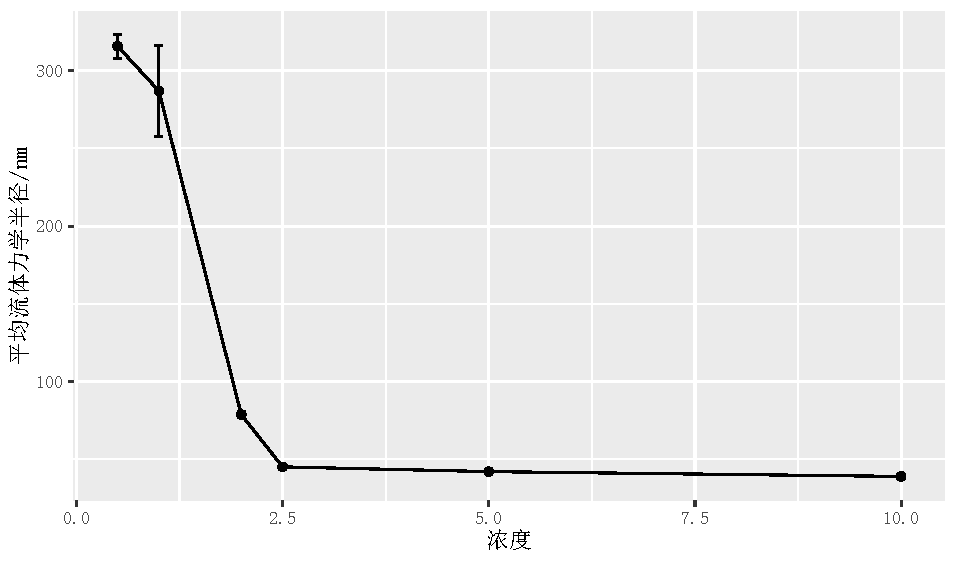
\includegraphics[width=0.7\linewidth]{Figure/test.pdf}
            \caption{}
            \label{fig:plot01}
        \end{figure}
        
    \section{开关表面活性剂}
    相比可分解表面活性剂分解不可恢复,开关表面活性剂的性质转变是可逆的,是可以调控的,
    例如,非离子表面活性剂就是一类传统的温度开关表面活性剂,当温度上升,其亲水性降低、
    表面活性降低,当温度恢复时其性质亦恢复。根据这些刺激响应的方式,可将开关表面活性剂分为:
    光开关、磁开关、温度开关、酸碱开关、\ce{CO2}开关及包含电化学方法和化学方法的氧化-还原开关表面活性剂\cite{秦勇2009}。
    
    \subsection{光开关表面活性剂}
    光开关表面活性剂在非极性疏水尾链或极性亲水头基中具有适当的显色基团\cite{张冤帝2017}。
    根据所需光照条件可将光开关表面活性剂分为两类:一类时热稳定型的,利用不同波长的光可
    调节表面活性剂的表面活性;另一类是不稳定的,只有用连续光照才可实现表面活性的转变。
    根据表面活性剂分子在转变中的变化特点,可将光开关表面活性剂分为顺反异构型、裂解-聚合型以及
    极性变化型开关表面活性\cite{张冤帝2017,李云霞2011}。
    顺反异构型开关表面活性剂是研究较早的光开关表面活性剂,其主要其结构有偶氮苯类、
    二苯乙烯类及烷基苯乙烯衍生物,此外,还有一些异构型光开关表面活性剂。异构型光开关表面活性剂
    见图\ref{fig:switchable-light}\cite{张冤帝2017,karthaus1996,shang2003,吕湘亮2018}。
    
    \begin{figure}[htbp]
        \centering
        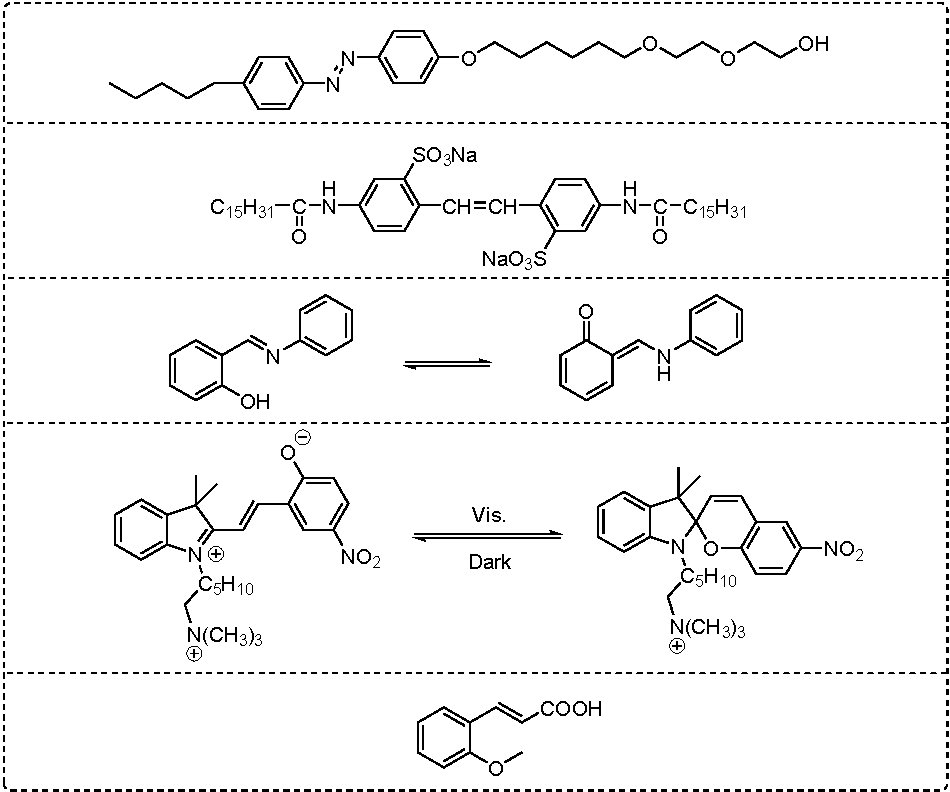
\includegraphics[width= \textwidth]{Figure/switchable-light.pdf}\\
        \caption{电化学方法实现氧化-还原开关表面活性剂:二茂铁基和联吡啶类开关表面活性剂}\label{fig:switchable-light}
    \end{figure}

    图\ref{fig:switchable-light} 几类异构型光开关表面活性剂\cite{张冤帝2017,karthaus1996,shang2003,吕湘亮2018}
    其中,偶氮型光开关表面活性剂研究较早,应用较广,一些光敏表面活性剂如偶氮类分解型及
    光照不可逆型不当归入光开关表面活性剂,刘清斌在其硕士论文中对光敏型表面活性剂做了总结\cite{刘清斌2018}。
    光开关表面活性剂或可在生物医药、环境修复及减阻传热等方面有所应用\cite{刘清斌2018},
    偶氮类光致异构化表面活性剂研究较多,我校王潮霞课题组\cite{chen2016}采用偶氮类阳离子表面活性剂BTAEAzo的光刺激开关实现绿色化的泡沫染整工艺。
    
    图 4 偶氮苯类阳离子表面活性剂的光致异构化\cite{chen2016}
    除光开关表面活性剂自生结构变化外,还可使用光相应分子与表面活性剂复配,构建光刺激相应系统,
    Zhao等\cite{zhao2016}将反式-邻甲氧基肉桂酸与N-甲基-N-乙基吡咯烷溴化物(C16MPB)碱性条件下
    自组装成为粘弹性蠕虫状胶束,经UV光照后反式-邻甲氧基肉桂酸构型转变,使体系转变成球形或棒状胶束。
    
    图 5 N-甲基-N-乙基吡咯烷溴化物(C16MPB)与邻甲氧基肉桂酸构成的光刺激响应体系\cite{zhao2016}。
    
    \subsection{磁开关表面活性剂}
    磁开关表面活性剂含有磁响应结构,有离子液体、螯合型以及多金属氧酸盐表面活性剂,此外,
    磁性有机分子表面活性剂是有待发展的新一类磁表面活性剂\cite{brown2015},Brown\cite{brown2015}对此类
    磁表面活性剂进行了综述,磁响应表面活性剂可用于蛋白质分离、水处理以及环境修复\cite{brown2015}。
    几类磁相应表面活性剂见图 6。
    
    图 6 三类主要的磁表面活性剂及一类潜在的磁表面活性剂\cite{brown2015,brown2012}
    
    \subsection{温度开关表面活性剂}
    非离子型表面活性剂是典型的温度开关表面活性剂,随温度升高其亲水性会逐渐下降,
    至浊点时亲水性显著降低,表面活性变差,而当温度降低后其又可恢复表面活性。Chu\cite{chu2011}等
    以PDAS为表面活性剂制备了一种温度响应凝胶,在30℃时形成球状或短棒状胶束,在40℃时则形成
    网络蠕虫状胶束,这是由于加热时疏水部分溶解度降低,从而形成网状交联凝胶。
    
    图 7 可切换温感凝胶
    \subsection{酸碱开关表面活性剂}
    酸碱开关表面活性剂即pH 开关表面活性剂,其通常含有羧酸、脒基、胍基等酸性或碱性基团,
    在pH 变化时,这些基团接受或给予质子,导致表面活性剂亲水或疏水性发生变化,从而调控
    表面活性剂的表面活性\cite{吕湘亮2018}。Lv\cite{lv2014}等合成一类酸碱开关Gemini表面活性剂,
    通过调控pH可实现制备的乳液在O/W乳液“开启”和W/O乳液“关闭”之间反转,见图 8。
    
    图 8 pH开关表面活性剂控制乳液类型转变
    此外,除通过pH调节表面活性剂亲疏水性改变体系性质,Brazdova\cite{李云霞2011,brazdova2008}等
    制得脂质体表面活性剂,通过pH 控制物质构象转化作为开关,见图 9。
    
    图 9 pH调节构象作为开关
    \subsection{\ce{CO2}/\ce{N2}开关表面活性剂}
    \ce{CO2}型开关表面活性剂其作用原理本质上和酸碱开关表面活性剂类似,利用\ce{CO2}气体的弱酸性,
    随着\ce{CO2}的通入和排出,体系的pH发生变化,从而引起体系内可离子化基团质子化或去质子化,
    导致亲疏水性发生变化,进而影响体系的表面活性。迄今为止,\ce{CO2}开关型表面活性剂主要包括
    脒/\ce{CO2}体系、胍/\ce{CO2}体系以及胺/\ce{CO2}体系\cite{梅平2016}。
    \ce{CO2}型开关表面活性剂采用\ce{CO2}作为调控手段,相比其他调控手段,价格便宜、无毒害且易除去等
    优点\cite{jessop2012},可应用于重油输送、土壤清洗、油砂分离及乳化聚合\cite{jessop2012}。
    早在开关表面活性剂概念提出之前,\ce{CO2}型开关表面活性剂已投入使用,Moore和Lefevre采用\ce{CO2}作为
    丁二烯/苯乙烯乳液聚合的开关表面能活性剂(见图 10.a),其中左式具有乳化作用而右式不具有乳化作用。
    
    图 10 较早应用及研究的\ce{CO2}型开关表面活性剂
    
    2006年,Jessop课题组\cite{liu2006science}提出一类脒类化合物可用于\ce{CO2}开关表面活性剂,
    此外,三级胺也可用于\ce{CO2}开关表面活性剂,但一级、二级胺则因为形成氨基甲酸酯在开关
    表面活性剂应用中有所难度\cite{jessop2012}。
    \subsection{氧化-还原开关表面活性剂}
    氧化还原型开关表面活性剂采用电化学方法或化学手段改变表面活性剂分子内部分结构,
    从而达到调整表面活性的目的。其中,前者研究最早且较为成熟的是二茂铁基表面活性剂
    ,其包含阳离子-两性离子可逆转换和阴离子-两性离子可逆转换两类\cite{李云霞2011}。
    图\ref{fig:switchable-redox-cp2fe}中前者是一类二茂铁基表面活性剂。但二茂铁基开关表面活性剂所需使用的二茂铁基团
    价格对该类表面活性剂的使用有所限制。
    
    \begin{figure}[htbp]
        \centering
        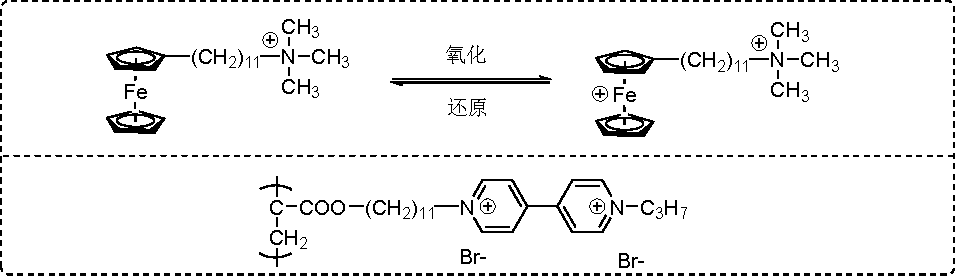
\includegraphics[width= \textwidth]{Figure/switchable-cp2fe.pdf}\\
        \caption{电化学方法实现氧化-还原开关表面活性剂:二茂铁基和联吡啶类开关表面活性剂}\label{fig:switchable-redox-cp2fe}
    \end{figure}
   
    此外,甲基紫类结构,即联吡啶类结构的表面活性剂也是一类良好的氧化-还原表面活性剂,
    但此类表面活性剂具有高毒性,如氯化二甲基联吡啶(即百草枯主要成分,一种高度植物农药)。
    
    除以上电化学方法的氧化还原表面活性剂之外,含二硫键结构的表面活性剂可在如含巯基试剂作用下断裂,
    从而改变分子结构。
    
    图 12 二硫键型氧化-还原开关表面活性剂
    最后,含硒表面活性剂作为一种新型的氧化-还原开关表面活性剂,Kong等\cite{kong2016redox}利用
    \ce{H2O2}将硒醚氧化为硒亚砜,使尾链亲水性增加,且在\ce{Na2SO3}等还原条件下又可恢复原结构。
    
    图 13 含硒氧化-还原表面活性剂的可逆转化\cite{kong2016redox}
    除以上类型的开关表面活性剂之外,还有酶催化\cite{ku2011}的开关表面活性剂有待讨论。
    

    \section{论文的目的与创新}
    云计算作为分布式技术的当前表现形式,通过将众多节点资源整合,以冗余、去
    中心化的分布式模式,实现传统技术中需要大型机才能解决的海量信息问题。一
    言而概之,“人多力量大”。在上述传统网络中,当节点总数达到数千乃至万数量级时,上层链路的聚合带宽
    将不断提高,从而对核心交换机、接入路由器、边界路由器的指标提出了极高的
    要求。以至于少数核心网络设备,成为整个网络中的高价格、高性能单点。一方
    面与原本追求低成本、分布化、去中心化的云技术设计理念背道而驰,另一方面
    也降低了网络的健壮性。因而本文所做工作对数据中心的网络基础设施而言,具
    有较大应用价值。
    
    %%%%%%%%%%%%%%%%%%%%%%%%%%%%%%%%%%%%%%%%%%%%%%%%%%%%%%%%%%%%%%%%%%%%%%%%%%%%%%%
    \chapter{实验部分}\label{chapter:experiment}
    \section{实验仪器与试剂}
        \begin{table}[htp]
        \centering
        \begin{tabular}{ccc}
            \toprule
            \textbf{仪器/试剂} & \textbf{规格/型号} & \textbf{生产厂家} \\
            \midrule
            硒   &  RG  & 阿达玛斯试剂 \\
s          硼氢化钠  & AR  & 上海化学试剂有限公司 \\
            1-溴代十二烷  & CP & 国药集团化学试剂有限公司 \\
            3-溴丙醇 & java.math.和具体值有关 & 国药集团化学试剂有限公司 \\
            氯磺酸  & java.math.B值有关 & 国药集团化学试剂有限公司 \\
            硫酸钠  & java.math.B值有关 & 国药集团化学试剂有限公司 \\
            亚硫酸钠  & java.math.B值有关 & 国药集团化学试剂有限公司 \\
            旋转蒸发器  & java.math.B值有关 & 国药集团化学试剂有限公司 \\
            超声波清洗器  & java.math.B值有关 & 国药集团化学试剂有限公司 \\
            核磁共振谱仪  & java.math.B值有关 & 国药集团化学试剂有限公司 \\
            双氧水  & java.math.B值有关 & 国药集团化学试剂有限公司 \\
            电子分析天平  & java.math.B值有关 & 国药集团化学试剂有限公司 \\
            液相色谱质谱联用仪  & java.math.B值有关 & 国药集团化学试剂有限公司 \\
            超级恒温水浴  & java.math.B值有关 & 国药集团化学试剂有限公司 \\
            \bottomrule
        \end{tabular}
        \caption{实验仪器与试剂}\label{table:实验仪器与试剂}
    \end{table}
    生活中,常出现初次见面的陌生人却拥有双方都认识的共同熟人,于是大家时常
    会感叹:“这世界真小!”。这种现象被称为``小世界现象'',后又称为``六度
    分割理论''。
    
    1909年,现代无线电之父Guglielmo Marconi在其诺贝尔奖致辞中讨论了覆盖整个地球所需
    的无线电中继站数目,并根据他的实验结果计算出平均需要$5.83$(近似为$6$)个中继站
    \cite{marconi1909nobel}。这个结论,被认为是``六度分割理论''中的常数$6$的最早出处
    \cite{barabasi2003linked}。
    
    \section{含硒表面活性剂的合成}
    \subsection{含硒表面活性剂的合成路线}
    \begin{figure}[htbp]
        \centering
        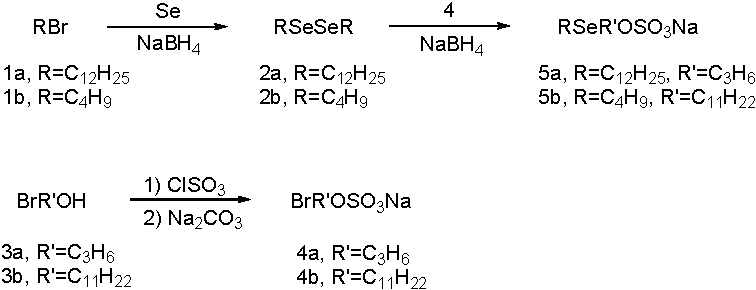
\includegraphics[]{Figure/synthesis.pdf}\\
        \caption{含硒表面活性剂的合成路线}\label{fig:synthesis}
    \end{figure}
    
    在刻画复杂网络结构的统计特性上有三个重要的指标:平均路径长度(average
    path length)、聚类系数(clustering coefficient)和度分布(degree
    distribution)。事实上,Watts和Strogatz提出小世界网络模型的初衷,就是
    
    \section{囊泡的构筑}
    
    想建立一个既具有类似随机图的较小的平均路径长度,又具有类似规则网络的较
    大的聚类系数的网络模型。
    
    \section{囊泡的性质研究}
    
    \begin{definition}[平均路径长度]
        网络的平均路径长度$L$定义为任意两个节点之间的距离的平均值,即
        \begin{equation}\label{eq:avarage_path_lentgh}
        L = \frac{2}{N(N+1)}\sum_{i\geq j}d_{ij}
        \end{equation}
        其中$N$为网络节点数。网络的平均路径长度也称为网络的特征路径长度。
    \end{definition}
    
    注意,为了便于数学处理,在公式\eqref{eq:avarage_path_lentgh}中包含了节
    点到其自身的距离(该距离为零)。如果不考虑节点到其自身的距离,那么公式
    \eqref{eq:avarage_path_lentgh}的右端需要乘以因子$(N+1)/(N-1)$。在实际应
    用中,该差别可以忽略不计。
    
    \begin{definition}[整体聚类系数]
        整体集聚系数的定义建立在闭三点组(邻近三点组)之上。假设网络中有一部分
        节点是两所有的连通三点组。整体集聚系数定义为
        一个网络中所有闭三点组的数量与所有连通三点组(无论开还是闭)的总量之比,
        即
        \[
        C_{total}=\frac{3\times G_{\triangle}}{3 \times G_{\triangle} + G_{\wedge}}
        \]
        其中$C_{total}$表示网络的整体聚类系数,$G_{\triangle}$表示该网络中闭三
        点组的个数,$G_{\wedge}$表示该网络中开三点组的个数\cite{luce1949method}。
    \end{definition}
    
    \begin{definition}[局部聚类系数]
        从几何特性上看,上式的一个等价定义为:
        \begin{equation}\label{eq:clustering_coefficient_triangle}
        C_i = \frac{\text{与节点$i$相连的三角形的数量}}{\text{与节点$i$相连
                的三元组的数量}}
        \end{equation}
        其中,与节点$i$相连的三元组是指由节点$i$和其两个邻居节点构成的组合。
    \end{definition}
    
   %%%%%%%%%%%%%%%%%%%%%%%%%%%%%%%%%%%%%%%%%%%%%%%%%%%%%%%%%%%%%%%%%%
    \chapter{实验结果与讨论}\label{chapter:results}
    \section{表面活性剂的结构表征}
    the fox jumps over the lazy dog.
        
    %%%%%%%%%%%%%%%%%%%%%%%%%%%%%%%%%%%%%%%%%%%%%%%%%%%%%%%%%%%%%%%%%%%%%%%%%%%%%%%
    % 学位论文的正文应以《结论》作为最后一章
    \chapter{结论与展望}\label{chapter:concludes}
    
    本文在第\ref{chapter_smallworld}章中,通过\cite{newman2001structure}考虑数据中心网络布局构建中的最大度限制
    问题,提出了符合数据中心网络基本要求的DS小世界模型,并分析了它的性质。随后提出
    SIDN,将DS模型映射到具体的网络结构中,并分析了所构成网络的平均直径、网络总带宽、
    对故障的容错能力等各项网络性能。
    
    分析与仿真实验证明,SIDN网络具有很好的扩展能力,网络总带宽与网络规模成
    近似线性增长的关系;具有很强的容错能力,链路损坏与节点损坏几乎无法破坏
    网络的联通性,故障率对网络性能的影响与破坏节点/链路占总资源比率线性相关。
    
    随后在第\ref{chapter_scalefree}章中,分析了无尺度网络在数据中心网络构建应用中的
    理论方面问题。对Scafida \cite{gyarmati2010scafida}文中所述在最大度限制的情况下运
    用BA算法构造的网络并不会损失无尺度性质的观点,进行了深入的分析,并指出了该论点的
    局限性。
    
    在给出了在引入节点最大度限制之后,利用分治和递归的思想,对无尺度网络
    进行多层构建,对所构造的网络进行度-度相关性,以及聚类性分析。
    
    \begin{table}
        \centering
        \begin{tabular}{cccp{38mm}}
            \toprule
            \textbf{文档域类型} & \textbf{Java类型} & \textbf{宽度(字节)} & \textbf{说明} \\
            \midrule
            BOOLEAN  & boolean &  1  & \\
            CHAR     & char    &  2  & UTF-16字符 \\
            BYTE     & byte    &  1  & 有符号8位整数 \\
            SHORT    & short   &  2  & 有符号16位整数 \\
            INT      & int     &  4  & 有符号32位整数 \\
            LONG     & long    &  8  & 有符号64位整数 \\
            STRING   & String  &  字符串长度  & 以UTF-8编码存储 \\
            DATE     & java.util.Date & 8 & 距离GMT时间1970年1月1日0点0分0秒的毫秒数 \\
            BYTE\_ARRAY & byte$[]$ & 数组长度 & 用于存储二进制值 \\
            BIG\_INTEGER & java.math.BigInteger & 和具体值有关 & 任意精度的长整数 \\
            BIG\_DECIMAL & java.math.BigDecimal & 和具体值有关 & 任意精度的十进制实数 \\
            \bottomrule
        \end{tabular}
        \caption{测试表格}\label{table:test5}
    \end{table}
    
    表\ref{table:test5}用于测试表格。随后分析了无尺度网络构造过程中,交换机节点与数
    据节点的角色区别,分析了两者在不同比率下形成的网络形态,以及对网络性能造成的影响。
    
    通过理论分析和仿真实验,分析并找出比率因子q的最佳取值。此外,无尺度现象
    的引入提高了网络的聚类系数,从而在不失灵活性可靠性的基础上,进一步提升
    了网络的性能。
    
    在第\ref{chapter_random}章中,将关注点转移到交换机本身。由于图论难以描述数据中心
    网络中的交换设备,因此放弃基于图的抽象模型,转而基于多维簇划分的思想,提出并设计
    了WarpNet网络模型。
    
    该网络模型突破了基于图描述的局限性,并对网络的带宽等指标进行理论分析并
    给出定量描述。最后对比了理论分析、仿真测试结果,并在实际物理环境中进系
    真实部署,通过6节点的小规模实验以及1000节点虚拟机的大规模实验,表明该模
    型的理论分析、仿真测试与实际实验吻合,并在网络性能、容错能力、伸缩性灵
    活性方面得到了进一步的提升。
    
    在第\ref{chapter_experiments}章中,针对网络模型研究这一类工作的共性,设计构造通
    用验证平台系统。以海量虚拟机和虚拟分布式交换机的形式,实现了基于少量物理节点,对
    大规模节点的模拟。其模拟运行的过程与真实运行在实现层面完全一致,运行的结果与真实
    环境线性相关。除为本文所涉若干网络模型提供验证外,可进一步推广到更为广泛的领域,
    为各种网络模型及路由算法的研究工作,提供分析、指导与验证。
    
    % 参考文献。应放在\backmatter之前。
    % 推荐使用BibTeX,若不使用BibTeX时注释掉下面一句。
    %\nocite{*}
    \bibliography{bachelor}
    % 不使用 BibTeX
    %\begin{thebibliography}{2}

    %%%%%%%%%%%%%%%%%%%%%%%%%%%%%%%%%%%%%%%%%%%%%%%%%%%%%%%%%%%%%%%%%%%%%%%%%%%%%%%
    % 致谢,应放在《结论》之后
    \begin{acknowledgement}
        首先感谢我的母亲韦春花对我的支持。其次感谢我的导师陈近南对我的精心指导和热心帮助。接下来,
        感谢我的师兄茅十八和风际中,他们阅读了我的论文草稿并提出了很有价值的修改建议。
        
        最后,感谢我亲爱的老婆们:双儿、苏荃、阿珂、沐剑屏、曾柔、建宁公主、方怡,感谢
        你们在生活上对我无微不至的关怀和照顾。我爱你们!
    \end{acknowledgement}
    s
    \begin{appendix}
    \chapter{彩色插图}
    \begin{figure}[htbp]
        \centering
        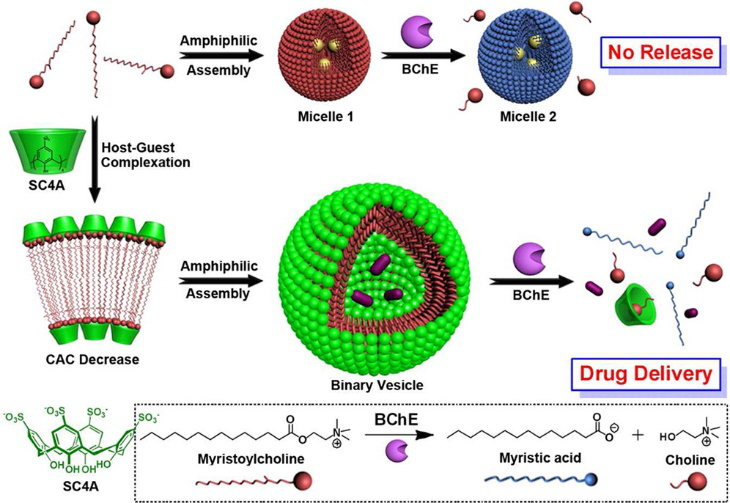
\includegraphics[width= 0.55\textwidth]{Figure/Ch1-SC4A}\\
        \caption{肉豆蔻酰胆碱在SC4A空白及存在下的两亲自组装示意图}
    \end{figure}
    \end{appendix}
    %%%%%%%%%%%%%%%%%%%%%%%%%%%%%%%%%%%%%%%%%%%%%%%%%%%%%%%%%%%%%%%%%%%%%%%%%%%%%%%
\end{document}